\documentclass[handout]{beamer}
%\usepackage[margin=1in]{geometry}
\usepackage{amsthm,amsmath,amsfonts,hyperref,graphicx,color,multicol}
\usepackage{enumitem,tikz}

%%%%%%%%%%
%Beamer Template Customization
%%%%%%%%%%
\setbeamertemplate{navigation symbols}{}
\setbeamertemplate{theorems}[ams style]
\setbeamertemplate{blocks}[rounded]

\definecolor{Blu}{RGB}{43,62,133} % UWEC Blue
\setbeamercolor{structure}{fg=Blu} % Titles

%Unnumbered footnotes:
\newcommand{\blfootnote}[1]{%
	\begingroup
	\renewcommand\thefootnote{}\footnote{#1}%
	\addtocounter{footnote}{-1}%
	\endgroup
}


%%%%%%%%%%
%Custom Commands
%%%%%%%%%%
\newcommand{\R}{\mathbb{R}}
\newcommand{\veca}{\vec{a}}
\newcommand{\vecb}{\vec{b}}
\newcommand{\vece}{\vec{e}}
\newcommand{\vecu}{\vec{u}}
\newcommand{\vecv}{\vec{v}}
\newcommand{\vecw}{\vec{w}}
\newcommand{\vecx}{\vec{x}}
\newcommand{\zerovector}{\vec{0}}

\newcommand{\ds}{\displaystyle}

\newcommand{\fn}{\insertframenumber}

\newcommand{\rank}{\operatorname{rank}}
\newcommand{\adj}{\operatorname{adj}}

\newcommand{\blank}[1]{\underline{\hspace*{#1}}}


%%%%%%%%%%
%Custom Theorem Environments
%%%%%%%%%%
\theoremstyle{definition}
\newtheorem{exercise}{Exercise}
\newtheorem{question}[exercise]{Question}
\newtheorem*{defn}{Definition}
\newtheorem*{exa}{Example}
\newtheorem*{disc}{Group Discussion}
\newtheorem*{nb}{Note}
\newtheorem*{recall}{Recall}
\renewcommand{\emph}[1]{{\color{blue}\texttt{#1}}}

\definecolor{Gold}{RGB}{237, 172, 26}
%Statement block
\newenvironment{statementblock}[1]{%
	\setbeamercolor{block body}{bg=Gold!20}
	\setbeamercolor{block title}{bg=Gold}
	\begin{block}{\textbf{#1.}}}{\end{block}}




\begin{document}
	\title{Math 324: Linear Algebra}
	\subtitle{Direct Proofs and Cases}
	\author{Mckenzie West}
	\date{Last Updated: \today}
\begin{frame}
\maketitle
\end{frame}

\begin{frame}{\insertframenumber}
	\begin{block}{\textbf{Last Time.}}
	\begin{itemize}[label=--]
		\item Proofs using Cases
	\end{itemize}
	\end{block}
\begin{block}{\textbf{Today.}}
	\begin{itemize}[label=--]
		\item If and only If Statements
		\item Contrapositive, Converse, and Inverse
	\end{itemize}
\end{block}
\end{frame}
\begin{frame}{\fn}
	\begin{exercise}[Warmup]
		Everyone at your table should read the pre-class exercise of another group member.  
		
		What do you like about their proof?  What do you think could be improved?
	\end{exercise}
	
	\begin{exercise}
		Discuss the advantages of using \LaTeX to typeset proofs.
		
		What are some challenges to using \LaTeX/Overleaf?
	\end{exercise}
\end{frame}

\begin{frame}[fragile]
\frametitle{\fn}
The general format of \emph{if and only if proofs} is to turn it into two smaller proofs:
\begin{center}
	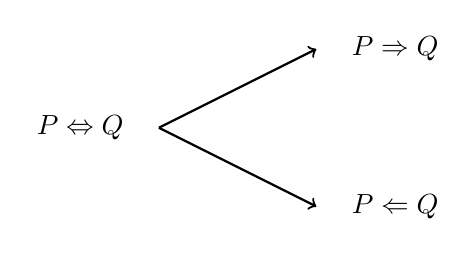
\begin{tikzpicture}
	\node at (-1,0) {$P\Leftrightarrow Q$};
	\draw [->, thick] (0,0) -- (2,1);
	\node at (3,1) {$P\Rightarrow Q$};
	\draw [->, thick] (0,0) -- (2,-1);
	\node at (3,-1) {$P\Leftarrow Q$};
	\end{tikzpicture}
\end{center}
We then prove both of these statements inside the larger proof.  Assume $P$ then show $Q$ is true.  Then do a total reset, forget everything that just happened.  Assume $Q$ is true then show $P$ is true.

\begin{block}{\textbf{Notation}}
	We read $P\Rightarrow Q$ as ``If $P$ then $Q$'' or as ``$P$ implies $Q$''.
\end{block}
\end{frame}
\begin{frame}{\fn}
\begin{exercise}\label{triv_sol}
	\textbf{Claim:} Let $A$ be a square matrix. The matrix $A$ is invertible if and only if the homogeneous system $A\vecx=\zerovector$ has only the trivial solution.
	
	\begin{enumerate}[label=(\alph*)]
		\item This is an if and only if proposition, i.e., it is of the form $P\Leftrightarrow Q$.  Identify the two statements $P$ and $Q$ as well as anything that will be referenced for the entire proof.
		\item Write the two propositions of the form $P\Rightarrow Q$ and $P\Leftarrow Q$ in full sentences.  In each case, what will you need to assume about $A$ and what will you need to prove?
		\item Do some scratch work for each of the directions of the proof so you know how the proof will go.
		\item Complete the proof of the claim on the worksheet.
	\end{enumerate}
\end{exercise}
\end{frame}

\begin{frame}{\fn}
	\begin{block}{\textbf{Brain Break.}}
		What’s the best class you’ve ever taken?
		\begin{center}
			
\includegraphics[width=2in]{images/class}
		\end{center}
	\end{block}
\end{frame}

\begin{frame}{\fn}
	\begin{defn}
		The \emph{contrapositive} of the statement $P\Rightarrow Q$ is the statement $\neg Q\Rightarrow \neg P$.  Recall that $\neg Q$ means ``not $Q$'' or ``the negation of $Q$''.
	\end{defn}
	\begin{exa}
		The contrapositive of the statement:
		\begin{center}
			If it is raining then the grass is wet.
		\end{center}
		is the statement:
		\begin{center}
			If the grass is not wet then it is not raining.
		\end{center}
	\end{exa}
	\begin{nb}
		The contrapositive of a statement is logically equivalent to the original statement.  Therefore, we can prove it instead.
	\end{nb}
\end{frame}
\begin{frame}{\fn}
	\begin{exercise}
		What is the contrapositive of this statement about $n\times n$ matrices $A$ and $B$?
			\begin{center}
				If $AB$ is an invertible matrix then $B$ is also invertible.
			\end{center}
	\end{exercise}
	\begin{nb}
		We can prove the contrapositive of this statement using the statement from Exercise \ref{triv_sol}.
	\end{nb}
\end{frame}
\begin{frame}{\fn}
	\begin{defn}
		The \emph{converse} of the statement $P\Rightarrow Q$ is the statement $Q\Rightarrow P$.
	\end{defn}
	\begin{exa}
		The converse of the statement:
		\begin{center}
			If it is raining then the grass is wet.
		\end{center}
		is the statement:
		\begin{center}
			If the grass is wet then it is raining.
		\end{center}
	\end{exa}
	\begin{nb}
		The converse is NOT logically equivalent to the original statement.  As you see in the example. There are other non-rain reasons that the grass could be wet.
	\end{nb}
\end{frame}
\begin{frame}{\fn}
\begin{exercise}
	What is the converse of the same statement about $n\times n$ matrices $A$ and $B$?
	\begin{center}
		If $B$ is a singular matrix then $AB$ is also singular.
	\end{center}
\end{exercise}
\begin{exercise}
	Find an example of square matrices $A$ and $B$ such that $AB$ is singular but $B$ is invertible.  Thus showing that the converse is false.
\end{exercise}
\end{frame}
\begin{frame}{\fn}
	\begin{defn}
		The \emph{inverse} of the statement $P\Rightarrow Q$ is the statement $\neg P\Rightarrow \neg Q$.
	\end{defn}
	\begin{exa}
		The inverse of the statement:
		\begin{center}
			If it is raining then the grass is wet.
		\end{center}
		is the statement:
		\begin{center}
			If it is not raining then the grass is not wet.
		\end{center}
	\end{exa}
	\begin{nb}
		The inverse is NOT logically equivalent to the original statement.  As you see in the example. There are other non-rain reasons that the grass could be wet. 
		But look, the inverse is the contrapositive of the converse, so they are logically equivalent.
	\end{nb}
\end{frame}
\begin{frame}{\fn}
\begin{exercise}
	What is the inverse of the same statement about $n\times n$ matrices $A$ and $B$?
	\begin{center}
		If $B$ is a singular matrix then $AB$ is also singular.
	\end{center}
\end{exercise}
	\begin{exercise}
		Does the same counterexample of the converse also function as a counterexample to the inverse?
	\end{exercise}
\end{frame}\begin{frame}{\fn}
\begin{block}{\textbf{Summary}}
	With the original statement $P\Rightarrow Q$, we have:
	\begin{center}
		\begin{tabular}{rcl}
			contrapositive & $\neg Q\Rightarrow \neg P$ & equivalent to $P\Rightarrow Q$\\
			converse & $Q\Rightarrow P$ & NOT equivalent to $P\Rightarrow Q$\\
			inverse & $\neg P\Rightarrow \neg Q$ & NOT equivalent to $P\Rightarrow Q$
		\end{tabular}
	\end{center}
\end{block}
\end{frame}
\begin{frame}{\fn}	
\begin{exercise}
	Consider the proposition:
	\begin{statementblock}{\textbf{Proposition.}}
		Let $A$ be a square matrix.
		If $A$ is a singular then $A\vecx=\zerovector$ has infinitely many solutions.
	\end{statementblock}
	\begin{enumerate}[label=(\alph*)]
		\item What is the contrapositive? 
		\item What is the converse? Is it True?
		\item What is the inverse? Is it True?
	\end{enumerate}
\end{exercise}
\end{frame}

\begin{frame}{\fn}
\begin{question}
	What is the relationship between if and only if statements and contrapositive/converse/inverse?
\end{question}
\end{frame}

\begin{frame}{\fn}	
\begin{exercise}
	Consider the proposition:
	
	\begin{statementblock}{\textbf{Proposition.}}
		Let $A$ and $B$ be a $m\times n$ matrices and $O_{m,n}$ the $m\times n$ zero matrix.
		If $A+B=A$ then $B=O_{m,n}$.
	\end{statementblock}
	\begin{enumerate}[label=(\alph*)]
		\item What is the contrapositive? 
		\item Do some scratch work toward either the original statement or the converse to convince yourself that they are true.
		\item What is the converse? Is it True?
		\item What is the inverse? Is it True?
	\end{enumerate}
\end{exercise}
\end{frame}
\end{document}

